\documentclass[a4paper,12pt]{article}
\usepackage{pgfplots}
\usepackage{listings}
\usepackage{xcolor}
\usepackage{float}
\usepackage{setspace}
\usepackage{graphicx}
\usepackage{indentfirst}
\usepackage{tikz}
\usetikzlibrary{positioning}
\usepackage{amsmath}
\usepackage{enumitem}
\newlist{steps}{enumerate}{1}
\setlist[steps, 1]{label = Step \arabic*:}
\newtheorem{theorem}{Theorem}[section]
\newtheorem{definition}{Definition}[section]
\newtheorem{summary}{Summary}[section]
\newtheorem{exmp}{Example}[section]
\tikzset{%
  every neuron/.style={
    circle,
    draw,
    minimum size=1cm
  },
  neuron missing/.style={
    draw=none, 
    scale=4,
    text height=0.333cm,
    execute at begin node=\color{black}$\vdots$
  },
}
\pgfplotsset{every axis/.append style={
                    axis x line=middle,    % put the x axis in the middle
                    axis y line=middle,    % put the y axis in the middle
                    axis line style={<->}, % arrows on the axis
                    xlabel={$x$},          % default put x on x-axis
                    ylabel={$y$},          % default put y on y-axis
                    label style={font=\tiny},
                    tick label style={font=\tiny}  
                    }}
\begin{document}
\title{Deep learning}
\author{Yanbo Liu}
\date{\today}
\maketitle
\begin{spacing}{2}
\pagenumbering{arabic}
\tableofcontents
\pagenumbering{arabic}
\end{spacing}
\begin{spacing}{2}
\section{Linear regression}
Let's say we have a lot of data points as shwon in figure 1, there are just some scatter points for use:
\begin{figure}[h]
\centering
\includegraphics[scale=0.5]{Figure_1.png}
\caption{Scatter points}
\label{scatter points}
\end{figure}

\paragraph{}Then if we want to fit a line into this picture, let's say y=x as shown in figure 2:
\begin{figure}[h]
\centering
\includegraphics[scale=0.5]{Figure_2.png}
\caption{A line y=x fit in scatter points}
\label{fitting line}
\end{figure}


 \paragraph{ } How can we know that it is the best line that we want to fit into the scatter point? We can have a horizontal line at the scatter points as shown in figure 3, and caculate the distance between each point and the horizontal line and sum them up:
\begin{figure}[h]
\centering
\includegraphics[scale=0.5]{Figure_3.png}
\caption{A line y=x fit in scatter points}
\label{horizontal line}
\end{figure}
\paragraph{ } In this figure the sum will be:
\begin{align}
S=(b-y_{1})+(b-y_{2})+(b-y_{3})+(b-y_{4})+\cdots+(b-y_{n})
\end{align}
\paragraph{ } where $b$ is 84, as shown in figure 3, there are some points whose y value is bigger than b, which makes the value of $b-y$ is negative, which is not what we want since it will make the overall fit than it really is.\\
\paragraph{ } So we can square each term to ensure each term is positive:
\begin{align}
S={(b-y_{1})}^2+{(b-y_{2})}^2+{(b-y_{3})}^2+\cdots+{(b-y_{n})}^2
\end{align}
\paragraph{ }This is our measure of how well this line fits the data.This is called \textbf{sum of squared residuals}, because the residuals are the differences between the real data and the line.In this case the final sum of squared residuals is 3362.
\paragraph{ }Let's get a new data set as shown in figure 4,in this case, the data point trend are much more smooth.So the fit is much better: 16
\newpage
\begin{figure}[h]
\centering
\includegraphics[scale=0.5]{Figure_4.png}
\caption{new data set}
\label{new fitting line}
\end{figure}
\paragraph{ } We can get ten different slop when the intercept doesn't change as shown in figure 5, the best point for the fit is when slope is 0 and intercept is 84 which is 16.\\
The best way to find the turning point is to find the point where the derivative of the function is 0.
\begin{figure}[h]
\centering
\includegraphics[scale=0.5]{Figure_5.png}
\caption{slope against sum of squared residuals}
\label{slope against sum of squared residuals}
\end{figure}
\paragraph{ } Corresponding code can be shown below:
\begin{tiny}
\begin{lstlisting}{tiny}[language=Python, caption=Simulated linear regression]
import matplotlib.pyplot as plt
import numpy as np
girls_grades = [85, 83, 83, 81, 84, 83, 83, 83, 83, 84]
boys_grades = [30, 29, 49, 48, 100, 48, 38, 45, 20, 30]
grades_range = [10, 20, 30, 40, 50, 60, 70, 80, 90, 100]

def function(data,data_range,a,b):
    #set the range of x
    x = np.linspace(0, 100, 100)
    y=a*x+b
    # fig=plt.figure()
    # if a==0:
    #     plt.plot(x,y,"-b",label="y={}".format(b))
    # else:
    #     plt.plot(x, y, "-b", label="y={}".format(b))
    # plt.scatter(data_range,data,label="scatter points")
    # plt.legend(loc="upper right")
    # plt.plot()
    # plt.show()
    sum=0
    for i in range(len(data_range)):
        x=data_range[i]
        y=a*x+b
        sum=sum+np.power(y-data[i],2)
    return sum


def linear_regression(slope_range,data,data_range,b):
    sum_lst=[]
    for i in range(len(slope_range)):
        print(i)
        sum_lst.append(function(data,data_range,slope_range[i],b))
    fig=plt.figure()
    plt.scatter(slope_range,sum_lst,label="slope against sum of squared residuals")
    plt.legend(loc="upper right")
    plt.plot()
    plt.show()
    print(sum_lst)
linear_regression([-6,-7,-5,-4,-3,-2,-1,0,1,2,3,4,5,6,7],girls_grades,grades_range,84)
\end{lstlisting}
\end{tiny}
\paragraph{ }But the situation above set the intercept to fixed value, the best fit will be found if we can use two independent variable they are slope and intercept of the function respectively as shown in figure 6
\begin{align}
&Q=\sum_{1}^n(y_{i}-(ax_{i}+b))^{2}
\end{align}

To get the derivative:
\begin{align}
&\frac{\partial Q}{\partial b}=-2\sum_{1}n(y_{i}-b-ax_{i})=0\\
&\frac{\partial Q}{\partial a}=-2a\sum_{1}n(y_{i}-b-ax_{i})x_{i}=0
\end{align}
\begin{figure}[h]
\centering
\includegraphics[scale=0.5]{Figure_6.jpg}
\caption{Two independent variables}
\label{Two independent variables}
\end{figure}
\section{Gradient Descent}
\paragraph{ }When we fit a line with \textbf{Linear Regression}, we optimize \textbf{Intercept} and \textbf{Slope}.When we use \textbf{Logistic Regression}, we optimize a \textbf{squiggle}, when we use T-SNE, we optimize \textbf{clusters}
\paragraph{ }First of all,set the slope of the line to a fixed value, then change the intercept as shown in figure 7.In this example we will still need to evaluate how well these line fit the data by using sum of squared residuals.
\begin{align}
&Q=\sum_{1}^n(y_{i}-(ax_{i}+b))^{2}
\end{align}
\newpage
\begin{figure}
\centering
\includegraphics[scale=0.5]{Figure_7.png}
\caption{Changeable intercepts}
\label{Changeable intecepts}
\end{figure}
In this case, relationship between sum of squared residuals and intercept is shown in figure 8. 
\begin{figure}[h]
\centering
\includegraphics[scale=0.5]{Figure_8.png}
\caption{Sum of squared residuals against intercept}
\label{Sum of squared residuals against intercept}
\end{figure}
\paragraph{ } But this is quite inconvenient if we have to take a lot of steps. So, as we did before, we can find the derivative of the quardratic function with respect to intercept.So here we can use gradient descent to get the sum.
\begin{align}
&\frac{\partial Q}{\partial b}=-2\sum_{1}n(y_{i}-b-ax_{i})=0\\
&\frac{\partial Q}{\partial a}=-2\sum_{1}n(y_{i}-b-ax_{i})x_{i}=0
\end{align}
Now that we have the derivative,gradient descent will use it to find where the sum of squared residuals is lowest.If we use \textbf{Linear Regression},We just simply find the lowest slope of the curve. In contrast,\textbf{Gradient Descent} finds the minimum value by taking steps from initial guess until it reaches the best value,which make \textbf{Gradient Descent} very useful when it not very easy to find the point where the derivative is 0.\\
Also, the closer we get to the optimal value, the closer we get to the best value.That means if the slope is getting closer to 0 then we should use baby steps otherwise we should use big steps.\\
The \textbf{Step size} can be determined by multiplying the slope by \textbf{Learning Rate} as shown in figure 9:
\begin{figure}
\centering
\includegraphics[scale=0.5]{Figure_9.png}
\caption{Gradient Descent}
\label{Gradient Descent}
\end{figure}
\\And in this case, the Learning rate we use is 0.00001,otherwise it is diverged. 
\newpage
\begin{summary}
So,we can use following orders to implement gradient descent:
\begin{steps}
  \item Take the derivative of the \textbf{Loss Function} for each parameter in it.In fancy Machine Learning Lingo,take the Gradient of the Loss function.
  \item Pick random values for the parameters
  \item Plug the parameter values into the derivatives(\textbf{Gradient})
  \item Caculate the step sizes:Step size=$Slope*Learning Rate$
  \item Caculate the new parameters:\textbf{New parameters=Old Parameter-Step Size}
\end{steps}
\textbf{Learning Rate} is quite important in gradient descent, if it was set to very high value,it will cause divergence as shown in figure 10:
\begin{figure}
\centering
\includegraphics[scale=0.5]{Figure_10.png}
\caption{Divergence of Gradient Descent}
\label{Divegerence of Gradient Descent}
\end{figure}
\end{summary}
\paragraph{ }Corresponding code:
\begin{tiny}
\begin{lstlisting}{tiny}[language=Python, caption=Gradient Descent]
import matplotlib.pyplot as plt
import numpy as np
import random
grades=[]
grades_range=[]
for i in range(1000):
    grades.append(random.randint(50,100))
    grades_range.append(random.randint(0,50))
Learning_rate=0.001

# derivative of sum of squared residuals with respect to intercept
def d_intercept(data_y,b,a,data_x):
    return -2*(data_y-(b+a*data_x))

# derivative of sum of squared residuals with respect to slope
def d_slope(data_y,b,a,data_x):
    return -2*data_x*(data_y-(b+a*data_x))
a=10
b=0
# gradient descent using recursion
def gradient_descent_recursion(data_range,data,a,b,learning_rate,counter=0):
    count=0
    x=np.linspace(0,100,100)
    y=a*x+b
    # figure=plt.figure()
    # if a==0:
    #     plt.plot(x,y,label="y={}".format(b))
    # elif b==0:
    #     plt.plot(x,y,label="y={}x".format(a))
    # else:
    #     plt.plot(x, y, label="y={}x+{}".format(a,b))
    # plt.scatter(data_range,data,label="data set")
    # plt.legend(loc="upper right")
    # plt.plot()
    # plt.show()
    slope_slope=0
    slope_intercept=0
    for i in range(len(data)):
        slope_intercept=slope_intercept+d_intercept(data[i],b,a,data_range[i])
        slope_slope=slope_slope+d_slope(data[i],b,a,data_range[i])
    step_size_intercept=learning_rate*slope_intercept
    step_size_slope=learning_rate*slope_slope
    new_intercept=b-step_size_intercept
    new_slope=a-step_size_slope
    print("step_size_intercept:",step_size_intercept)
    print("step_size_slope:",step_size_slope)
    print("\n\n")
    print("counter:",counter)
    if abs(step_size_slope)<0.01 or abs(step_size_intercept)<0.001 or counter>1000:
        print("The final slope is:",a)
        print("The final intercept:",b)
        print("The count of recursion is :",counter)
        figure=plt.figure()
        if a==0:
            plt.plot(x,y,label="y={}".format(b))
        elif b==0:
            plt.plot(x,y,label="y={}x".format(a))
        elif b<0:
            plt.plot(x,y,label="y={}x-{}".format(a,abs(b)))
        else:
            plt.plot(x, y, label="y={}x+{}".format(a,b))
        plt.scatter(data_range,data,label="data set")
        plt.legend(loc="upper right")
        plt.plot()
        plt.show()
        return
    else:
        gradient_descent_recursion(data_range,data,new_slope,new_intercept,learning_rate,counter+1)


# gradient descent using iteration
def gradient_descent_iteration(data_range,data,a,b,learning_rate):
    temp_intercept=b
    temp_slope=a
    for i in range(1000):
        slope_slope = 0
        slope_intercept = 0
        for j in range(len(data)):
            slope_intercept = slope_intercept + d_intercept(data[j], temp_intercept, temp_slope, data_range[j])
            slope_slope = slope_slope + d_slope(data[j], temp_intercept, temp_slope, data_range[j])
        step_size_intercept = learning_rate * slope_intercept
        step_size_slope = learning_rate * slope_slope
        new_intercept = temp_intercept - step_size_intercept
        new_slope = temp_slope - step_size_slope
        temp_slope=new_slope
        temp_intercept=new_intercept
        if abs(step_size_slope) < 0.001 or abs(step_size_intercept) < 0.001:
            x = np.linspace(0, 100, 100)
            y = new_slope * x + new_intercept
            figure = plt.figure()
            if new_slope == 0:
                plt.plot(x, y, label="y={}".format(new_intercept))
            elif new_intercept == 0:
                plt.plot(x, y, label="y={}x".format(new_slope))
            elif new_intercept< 0:
                plt.plot(x, y, label="y={}x-{}".format(new_slope, abs(new_intercept)))
            else:
                plt.plot(x, y, label="y={}x+{}".format(new_slope, new_intercept))
            plt.scatter(data_range, data, label="data set")
            plt.legend(loc="upper right")
            plt.plot()
            plt.show()
            return
    print("The model is diverged!!!")



gradient_descent_iteration(grades_range,grades,a,b,Learning_rate)
gradient_descent_recursion(grades_range,grades,a,b,Learning_rate)
\end{lstlisting}
\end{tiny}
\section{Stochastic Gradient Descent}
\paragraph{ }\textbf{Stochastic Gradient Descent} is very similar to Gradient Descent,but instead of caculating sum of squared residuals it uses one sample or mini batch of samples per each step.It is very useful when we have a lot of datas and a lot of parameters.In these situations, regular gradient may not be computationally feasible.In supervised learning, eduach example is a pair consisting of an input object (typically a vector) and a \textbf{desired output} value (also called the supervisory signal). A supervised learning algorithm analyzes the training data and produces an inferred function, which can be used for mapping new examples.
\subsection{Supervised Learning}
\begin{theorem}
Supervised learning (SL) is the machine learning task of learning a function that maps an input to an output based on example input-output pairs.[1] It infers a function from labeled training data consisting of a set of training examples.
\end{theorem}
\paragraph{ }In Supervised learning, the correct output has already been given.It is basically a process of   modifying the weight for each step. For Supervised learning, it should obeyed following order:
\begin{steps}
  \item Initialize the weights
  \item Caculate the error from the difference between output and correct output
  \item Caculate the weights updates.
  \item Adjust the weight updates
  \item Repeat step 2 to 4 for all training data
  \item Repeat step 2 to 5 until the error reaches an acceptable level.\\
\end{steps}
\paragraph{ }Here is a simple figure of neural network as shown figure 10. And we just want to build a single layer neural network, so just ignore the Hidden layer.
\begin{center}

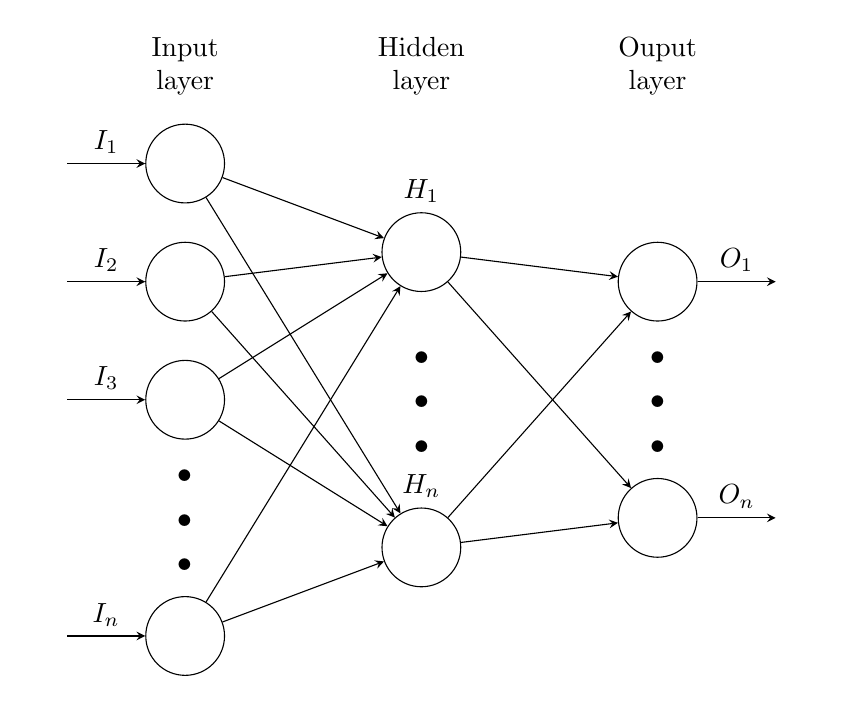
\begin{tikzpicture}[x=1.5cm, y=1.5cm, >=stealth]

\foreach \m/\l [count=\y] in {1,2,3,missing,4}
  \node [every neuron/.try, neuron \m/.try] (input-\m) at (0,2.5-\y) {};

\foreach \m [count=\y] in {1,missing,2}
  \node [every neuron/.try, neuron \m/.try ] (hidden-\m) at (2,2-\y*1.25) {};

\foreach \m [count=\y] in {1,missing,2}
  \node [every neuron/.try, neuron \m/.try ] (output-\m) at (4,1.5-\y) {};

\foreach \l [count=\i] in {1,2,3,n}
  \draw [<-] (input-\i) -- ++(-1,0)
    node [above, midway] {$I_\l$};

\foreach \l [count=\i] in {1,n}
  \node [above] at (hidden-\i.north) {$H_\l$};

\foreach \l [count=\i] in {1,n}
  \draw [->] (output-\i) -- ++(1,0)
    node [above, midway] {$O_\l$};

\foreach \i in {1,...,4}
  \foreach \j in {1,...,2}
    \draw [->] (input-\i) -- (hidden-\j);

\foreach \i in {1,...,2}
  \foreach \j in {1,...,2}
    \draw [->] (hidden-\i) -- (output-\j);

\foreach \l [count=\x from 0] in {Input, Hidden, Ouput}
  \node [align=center, above] at (\x*2,2) {\l \\ layer};
\end{tikzpicture}\\
Figure 10:{A simple Neural Network}
\end{center}
For Supervised Learning, it is a process of modifying the weights for each step and the desired output has already been fixed which can be expressed as following equations:
\begin{align}
&e_{i}=d_{i}-y_{i}\\
&\Delta w_{ij}=\alpha e_{i} x_{j}\\
&w_{ij} \quad \leftarrow w_{ij}+ \Delta w_{ij}
\end{align}
\paragraph{ }These equations can be also called \textbf{Delta rule}where $e$ is the error between the correct output and real output. And $d $ is the correct output, $y$ is the real output. $\alpha$ is the learning rate which is usually set between 0 and 1.\\

\paragraph{ }But the above equations are only correct when the activation function is linear function as shown in below in figure 11.
\begin{center}
\begin{tikzpicture}[scale=1, transform shape]
\begin{axis}[grid=none,
      mark = none,
      xmin = -10, ymin = -10,
      xmax = 17,ymax = 16,
      axis lines*=middle,
      enlargelimits=upper,
      clip=false,
      xtick={-10,-8,...,17},
      ytick={-10,-8,...,16}]
\addplot[blue, domain=0:14,restrict y to domain=0:18, samples=100]  {x} node[right,anchor=north west]{\scalebox{1.5}{$y=x$}};
\end{axis}
\end{tikzpicture}\\
Figure 11:{Linear activation equation}
\end{center}
Then we should consider about when activation function is not a linear function , for example if it is a sigmoid function as shown in figure 12.
\begin{center}
\begin{tikzpicture}[scale=1, transform shape]
\begin{axis}[grid=none,
      mark = none,
      xmin = -10, ymin = 0,
      xmax = 17,ymax = 1,
      axis lines*=middle,
      enlargelimits=upper,
      clip=false,
      xtick={-10,-8,...,17},
      ytick={0,0.5,1}]
\addplot[blue, domain=-10:10,restrict y to domain=0:1, samples=100]  {1/(1+exp(-x))} node[right,anchor=north west]{\scalebox{1.5}{$y=\frac{1}{1+e^{-x}}$}};
\end{axis}
\end{tikzpicture}\\
Figure 12: Sigmoid function
\end{center}
\paragraph{ }So in this case, the \textbf{Delta rule} is not useful anymore it should be transformed to another form called \textbf{generalized Delta rule} which can be expressed as equations:
\begin{align}
w_{ij} \quad \leftarrow w_{ij}+\alpha \delta e_{i} x_{j} 
\end{align}
\paragraph{ }In this experiment, a SGD method was used for supervised learning.And the number of training and mean errors were recorded to plot the graph as shown in figure 13:
\begin{figure}
\centering
\includegraphics[scale=0.5]{Figure_13.png}
\caption{Mean Error against Training number}
\label{Mean Errors against Training number}
\end{figure}
\section{Logistic Regression}
\paragraph{ }Logistic regression is basically like the linear regression, but a bit different. As shown in figure 14, we have a lot of scatter points but the corresponding y value is either 1 or 0 which represent some event that will happen or not in the real world.
\begin{figure}
\centering
\includegraphics[scale=0.5]{Figure_14.png}
\caption{data set}
\label{data set}
\end{figure}
\paragraph{ }And as we did in the linear regression, we try to add a fitting line as shown in figure 15:
\begin{figure}
\centering
\includegraphics[scale=0.5]{Figure_15.png}
\caption{add a fitting line}
\label{add a fitting line}
\end{figure}
\paragraph{ }It seems like that the fitting line is not relevant to all of these scatter points.But it actually looks like sigmoid function as shown below:
\begin{center}
\begin{tikzpicture}[scale=1, transform shape]
\begin{axis}[grid=none,
      mark = none,
      xmin = -10, ymin = 0,
      xmax = 17,ymax = 1,
      axis lines*=middle,
      enlargelimits=upper,
      clip=false,
      xtick={-10,-8,...,17},
      ytick={0,0.5,1}]
\addplot[blue, domain=-10:10,restrict y to domain=0:1, samples=100]  {1/(1+exp(-x))} node[right,anchor=north west]{\scalebox{1.5}{$y=\frac{1}{1+e^{-x}}$}};
\end{axis}
\end{tikzpicture}\\
Sigmoid function
\end{center}
\paragraph{ }The basic form of multiple linear regression is like this:
$y=\beta_{0}+\beta_{1}x_{1}+\beta_{2}x_{2}+\beta_{3}x_{3}+\cdots+\beta_{p}x_{p}$ which can be simplified into $\textbf{Y}=\textbf{X}\beta$ where,
\begin{align}
\textbf{Y}=\begin{bmatrix}
y_{1}\\
y_{2}\\
y_{n}
\end{bmatrix},\quad \textbf{X}=\begin{bmatrix}
1&x_{11}&x_{12}&x_{13}\cdots&x_{1p}\\
1&x_{21}&x_{22}&x_{23}\cdots&x_{2p}\\
1&x_{31}&x_{32}&x_{33}\cdots&x_{3p}\\
\vdots&\vdots&\vdots&\vdots&\vdots\\
1&x_{n1}&x_{n2}&x_{n3}\cdots&x_{np}
\end{bmatrix}
\end{align}
\paragraph{ }Substitute Y into the sigmoid function which can be expressed as $y=\frac{1}{1+exp(-x\beta)}$,the probability of positive is $P(Y=1)$ then the form of logistic regression comes up:
\begin{align}
P(Y=1)=\frac{1}{1+exp(-X\beta)}.
\end{align}
\paragraph{ }Now,before we figure out the value of $\beta$, we need to know a concept: \textbf{Likelihood function}
\subsection{Likelihood function}
\begin{definition}[Likelihood function]
In statistics, the likelihood function (often simply called the likelihood) measures the goodness of fit of a statistical model to a sample of data for given values of the unknown parameters. It is formed from the joint probability distribution of the sample, but viewed and used as a function of the parameters only, thus treating the random variables as fixed at the observed values.
\end{definition}
\paragraph{ }We usually use possibility to describe how possible an event that can happen, but we use likelihood function to describe with which parameter,the event is most likely to happen.which can be expressed in mathematical word:
\begin{itemize}
  \item which a parameter $\beta$ the possibility of an event which will happen is $P(x|\beta)$
  \item If we already an event will happen, the likelihood function of the parameter is $L(\beta|x);$
  \item $L(\beta|x)=P(x|\beta)$
\end{itemize}
\paragraph{ }One parameter $\beta$ is related to one value of likelihood function,when the value of $\beta$ changes ,$L(\beta|x)$will also change, when the value of likelihood function reaches the peak this at this value of parameter it is most reasonable.

\subsection{Loss function of Logistic Regression}
\paragraph{ }Before we talk about the logistic function we need to know the most likelihood estimation.In \textbf{binary classification}, when y is either 1 or 0, the combination can be used to show the possibility   that y can happen $P(y)=P(y=1)^{y}P(y=0)^{1-y}$
\begin{definition}[Binary Classification]Binary classification is the task of classifying the elements of a set into two groups on the basis of a classification rule. 
\end{definition}
\paragraph{ } Technically, the equation should be changed into $P(y|x,\beta)=P(y=1|\beta,x)^{y}[1-P(y=1|\beta,x)^{1-y}]$, then substitute $\frac{1}{1+exp(-x\beta)}$, then $ p(y|x,\beta)=(\frac{1}{1+exp(-x\beta)})^{y}(1-\frac{1}{1+exp(-x\beta)})^{1-y}$. we want to maximize the possibility of our samples, so we need to find the maximum value of the following equations:
\begin{align}
L(\beta|x)=\prod_{i=1}^{n}P(y_{i}|x_{i},\beta)=\prod_{i=1}^{n}p(y|x,\beta)=(\frac{1}{1+exp(-x_{i}\beta)})^{y_{i}}(1-\frac{1}{1+exp(-x_{i}\beta)})^{1-y_{i}}
\end{align}
\paragraph{ }It is hard to find the maximum vale of above equations, so we can use $log(L(\beta|x))=\sum_{i=1}^{n}([y_{i}log(\frac{1}{1+exp(-x_{i}\beta)})]+[(1-y_{i})log(1-\frac{1}{1+exp(-x_{i}\beta)})])$
\paragraph{ }In the \textbf{Linear Regression} section, we use $\sum_{1}^{n}(y_{i}-\hat{y_{i}})^{2}=\sum_{1}^{n}(y_{i}-x_{i}\beta)^{2}$,if logistic function use the same loss function it will be 
\begin{align}
Q=\sum_{1}^{n}(y_{i}-\frac{1}{1+exp(-x_{i}\beta)})^{2}
\end{align} 
\paragraph{ }unfortunately, it is not a convex function,it will have a lot of optimal local values,so the logistic function uses \textbf{log loss function}.
\paragraph{ }For \textbf{log loss}, it will be 
\begin{align}
J(\beta)=-logL(\beta)=-\sum_{i=1}^{n}[y_{i}logP(y_{i})+(1-y_{i})log(1-P(y_{i}))]
\end{align}
\paragraph{ }So for this equation, if i get x and corresponding y=0.6, but the real y is 1 so the loss will be log(0.6) and if the corresponding y=0.3, and the real y is 0 so the loss will be log(0.3).

\paragraph{ }We know that the derivative of sigmoid function is 
\begin{align}
f'(x)=f(x)(1-f(x))
\end{align}
\paragraph{ }substitute $f(x_{i}\beta)=\frac{1}{1+exp(-x_{i}\beta)}$ into $J(\beta)$
\begin{align}
J(\beta)=-\sum_{i=1}^{n}[y_{i}log(f(x_{i}\beta)))+(1-y_{i})log(1-f(x_{i}\beta))]
\end{align}
We know 
\begin{align}
\frac{\partial f(x_{i}\beta)}{\partial\beta_{j}}=f(x_{i}\beta)*(1-f(x_{i}\beta))*x_{ij}
\end{align}
\paragraph{ }Using chain rule,the derivative of loss function  can be simplified into:
\begin{align}
\frac{\partial J(\beta)}{\partial\beta_{j}}=\sum_{i=1}^{n}(\frac{1}{exp(-x_{i}\beta)}-y_{i})x_{ij}
\end{align}
\paragraph{ }Now we can use gradient descent as we talked before.Here is the following order:
\begin{itemize}
\item Initialize $\beta$ vector, which is known as $\theta_{0}$, then substitute it into current gradient
\item Use learning rate(step) $\alpha$ multiply the current gradient, and get the current step size $G$.
\item update $\theta_{0}$, the equation will be $ \theta{1}=\theta_{0}-\alpha G$
\item repeat the procedures above until the step size is very small( you can set the condition)
\end{itemize}
\end{spacing}
\end{document}